\fontsize{13px}{13px}\selectfont\justifying

\subsection{Sơ đồ triển khai}
\begin{figure}[h!]\fontsize{13px}{13px}\selectfont
\centering
		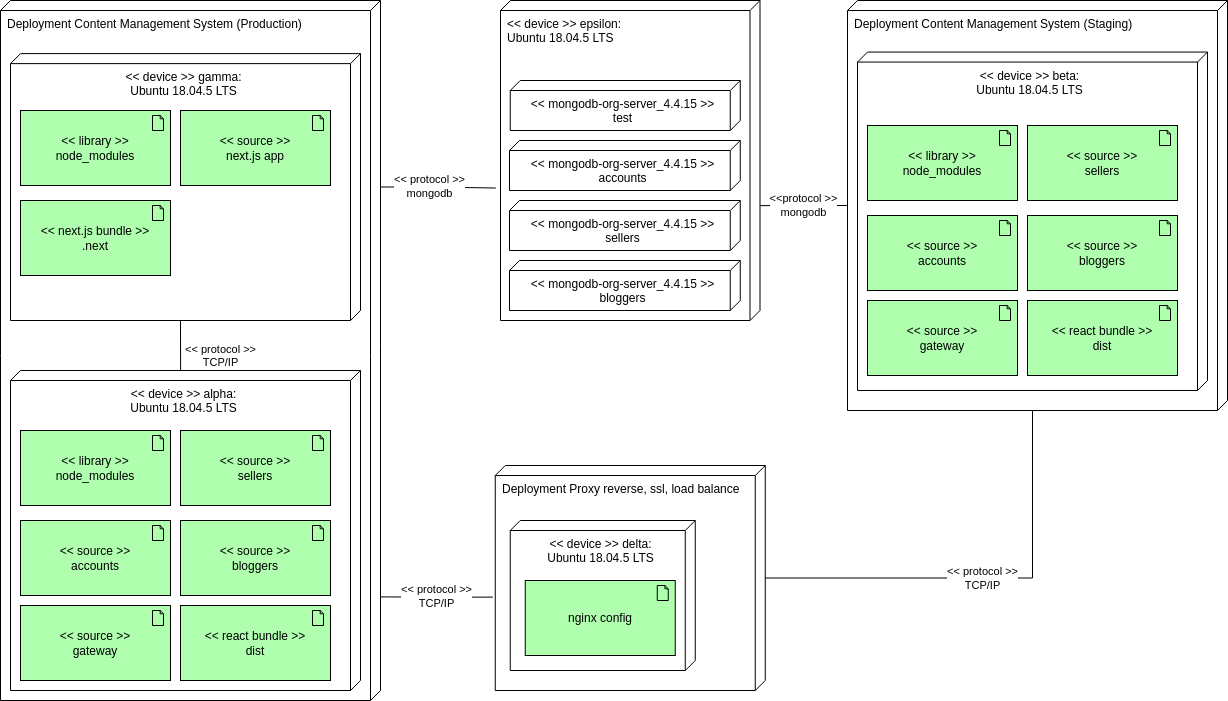
\includegraphics[width=\textwidth]{deployment}
		\caption{Sơ đồ triển khai tổng quát}
\justifying
Hệ thống cần tối thiểu 4 môi trường phát hành khác nhau. Trong môi trường \Gls{production} và môi trường \Gls{staging}, các thiết bị có thể nhân bản ra để phục vụ việc cân bằng tải thông qua thuật toán phân phối tải của máy chủ nginx.

Hệ thống sử dụng CI/CD của Github Actions giúp cho việc triển khai trở nên tự động và có thể sao lưu dự phòng tại mỗi phiên bản phát hành.

Github Actions cơ bản cung cấp chức năng kích hoạt đoạn mã triển khai của hệ thống khi có một hoạt động quản lý mã nguồn phù hợp với nội dung mà chúng ta đã cấu hình. Ví dụ như khi mã nguồn được gộp vào nhánh cho tên là \gls{production}, thì chạy mã triển khai \gls{production} ở phía máy chủ.
\end{figure}
